\section{Appendix} \label{sec:appx}

%\subsection{Discussion on nuisance component} \label{appx:nuisance}


\subsection{Proof of Lemma \ref{lemma:valid_selective_p}} \label{appx:proof_valid_selective_p}

We have 
\[
\bm \eta_j^\top {\bm X^s \choose \bm X^t} \mid
	\left \{  
	\cO_{\bm X^s, \bm X^t}
	=
	\cO_{\rm obs},
	\cQ_{\bm X^s, \bm X^t}
	=
	\cQ_{\rm obs}
	\right \} 
	\sim 
	{\rm TN} 
	\left (
	\bm \eta_j^\top 
	{\bm \mu^s \choose \bm \mu^t},
	\bm \eta_j^\top \Sigma \bm \eta_j,
	\cZ
	\right ),
\]
which is a truncated normal distribution with a mean $\bm \eta_j^\top {\bm \mu^s \choose \bm \mu^t}$,
 variance $\bm \eta_j^\top \Sigma \bm \eta_j$ in which $
\Sigma = 
\begin{pmatrix}
	\Sigma^s & 0 \\ 
	0 & \Sigma^t
\end{pmatrix}
$, and the truncation region $\cZ$ described in Sec. \ref{subsec:conditional_data_space}.
%
Therefore, under the null hypothesis,
\begin{align*}
	p_j^{\rm sel}
	\mid 
	\{ \cO_{\bm X^s, \bm X^t}
	=
	\cO_{\rm obs},
	\cQ_{\bm X^s, \bm X^t}
	=
	\cQ_{\rm obs}
	\}
	\sim {\rm Unif}(0, 1).
\end{align*} 
%
Thus,
%
$
	\mathbb{P}_{\rm H_{0, j}}  \Big (
	p_j^{\rm sel} \leq \alpha
	\mid 
	\cO_{\bm X^s, \bm X^t}
	=
	\cO_{\rm obs},
	\cQ_{\bm X^s, \bm X^t}
	=
	\cQ_{\rm obs}
	\Big) = \alpha, \forall \alpha \in [0, 1].
$

Next, we have 
%
\begin{align*}
	&\mathbb{P}_{\rm H_{0, j}}  \Big (p_j^{\rm sel} \leq \alpha \mid \cO_{\bm X^s, \bm X^t} = \cO_{\rm obs} \Big ) \\ 
	&= 
	\int
	\mathbb{P}_{\rm H_{0, j}}  \Big (p_j^{\rm sel} \leq \alpha \mid \cO_{\bm X^s, \bm X^t} = \cO_{\rm obs},  \cQ_{\bm X^s, \bm X^t} = \cQ_{\rm obs} \Big ) ~
	\mathbb{P}_{\rm H_{0, j}}  \Big (\cQ_{\bm X^s, \bm X^t} = \cQ_{\rm obs} \mid \cO_{\bm X^s, \bm X^t} = \cO_{\rm obs} \Big ) d\cQ_{\rm obs} \\ 
	&= 
	\int \alpha 
	~ \mathbb{P}_{\rm H_{0, j}}  \Big (\cQ_{\bm X^s, \bm X^t} = \cQ_{\rm obs} \mid \cO_{\bm X^s, \bm X^t} = \cO_{\rm obs} \Big ) d\cQ_{\rm obs} \\ 
	& = 
	\alpha 
	\int \mathbb{P}_{\rm H_{0, j}}  \Big (\cQ_{\bm X^s, \bm X^t} = \cQ_{\rm obs} \mid \cO_{\bm X^s, \bm X^t} = \cO_{\rm obs} \Big ) d\cQ_{\rm obs} \\ 
	& = 
	\alpha.
\end{align*} 
%
Finally, we obtain the result in Lemma \ref{lemma:valid_selective_p} as follows:
%
\begin{align*}
	\mathbb{P}_{\rm H_{0, j}}  \Big (p_j^{\rm sel} \leq \alpha \Big ) 
	& = \sum \limits_{\cO_{\rm obs}}
	\mathbb{P}_{\rm H_{0, j}}  \Big (p_j^{\rm sel} \leq \alpha \mid \cO_{\bm X^s, \bm X^t} = \cO_{\rm obs} \Big ) ~
	\mathbb{P}_{\rm H_{0, j}}  \Big (\cO_{\bm X^s, \bm X^t} = \cO_{\rm obs} \Big ) \\ 
	& = \sum \limits_{\cO_{\rm obs}} \alpha ~ \mathbb{P}_{\rm H_{0, j}}  \Big (\cO_{\bm X^s, \bm X^t} = \cO_{\rm obs} \Big ) \\ 
	& = \alpha \sum \limits_{\cO_{\rm obs}} \mathbb{P}_{\rm H_{0, j}}  \Big (\cO_{\bm X^s, \bm X^t} = \cO_{\rm obs} \Big ) \\ 
	& = \alpha.
\end{align*}



%========================

\subsection{Proof of Lemma \ref{lemma:data_line}} \label{appx:proof_lemma_data_line}

According to the second condition in \eq{eq:conditional_data_space}, we have 
%
\begin{align*}
	\cQ_{\bm X^s, \bm X^t} & =  \cQ_{\rm obs} \\ 
	\Leftrightarrow 
	\left ( 
	I_{n_s + n_t} - 
	\bm b
	\bm \eta_j^\top \right ) 
	{\bm X^s \choose \bm X^t}
	& = 
	\cQ_{\rm obs}\\ 
	\Leftrightarrow 
	{\bm X^s \choose \bm X^t}
	& = 
	\cQ_{\rm obs}
	+ \bm b
	\bm \eta_j^\top  
	{\bm X^s \choose \bm X^t}.
\end{align*}
%
By defining 
$\bm a = \cQ_{\rm obs}$,
$z = \bm \eta_j^\top {\bm X^s \choose \bm X^t}$, and incorporating the first condition of \eq{eq:conditional_data_space}, we obtain Lemma \ref{lemma:data_line}. 



%========================

\subsection{Proof of Lemma \ref{lemma:cZ_1}} \label{appx:proof_lemma_cZ_1}



The proof is constructed based on the results presented in \cite{duy2021exact}, in which the authors introduced an approach to characterize the event of OT by using the concept of \emph{parametric linear programming}.
%
Let us re-written the OT problem between the source and target domain in \eq{eq:ot_problem} as:
%
\begin{align*}
	\hat{\bm t} = \argmin \limits_{\bm t \in \RR^{n_s n_t}} ~~ & 
	\bm t^\top \bm c(\bm X^s, \bm X^t) \\
	\text{s.t.} ~~
	& H \bm t = \bm h, ~\bm t \geq \bm 0, \nonumber
\end{align*}
%
where $\bm t = {\rm {vec}}(T)$,
%
$
	\bm c(\bm X^s, \bm X^t) 
	= {\rm {vec}} (C(\bm X^s, \bm X^t)) 
	= \left [ \Omega {\bm X^s \choose \bm X^t} \right] \circ \left [ \Omega {\bm X^s \choose \bm X^t} \right]
$,
\[
\Omega = {\rm hstack}\left ( 
	I_{n_s} \otimes \bm 1_{n_t}, - \bm 1_{n_s} \otimes I_{n_t} \right ) 
\in \RR^{n_s n_t \times (n_s + n_t)},
\]
${\rm vec}(\cdot)$ is an operator that transforms a matrix into a vector with concatenated rows, the operator $\circ$ is element-wise product, $\rm hstack(\cdot, \cdot)$ is horizontal stack operation, $I_n \in \RR^{n \times n}$ is the identity matrix, and $\bm 1_m \in \RR^m$ is a vector of ones.
%
The matrix $H$ is defined as 
$ H = \left( H_r ~ H_c \right )^\top \in \RR^{(n_s + n_t) \times n_s n_t}$ in which 
%
\begin{align*}
	H_r = 
	\begin{bmatrix}
		1 ~ \ldots ~  1 & 0 ~ \ldots ~  0 & \ldots & 0 ~ \ldots ~  0 \\
		0 ~ \ldots ~  0 & 1 ~ \ldots ~  1 & \ldots & 0 ~ \ldots ~  0 \\
		 ~ \ldots ~   &  ~ \ldots ~   & \ldots &  ~ \ldots ~   \\
		0 ~ \ldots ~  0 & 0 ~ \ldots ~  0 & \ldots & 1 ~ \ldots ~  1 \\
	\end{bmatrix} \in \RR^{n_s \times n_s n_t}
\end{align*} 
%
that performs the sum over the rows of $T$ and 
%
\begin{align*}
	 H_c = 
	\begin{bmatrix}
		I_{n_t} & I_{n_t} & \ldots & I_{n_t}
	\end{bmatrix} \in \RR^{n_t \times n_s n_t}
\end{align*}
%
that performs the sum over the columns of $T$, and $\bm h = \left (\bm 1_{n_s}/{n_s} ~ \bm 1_{n_t}/{n_t} \right)^\top \in \RR^{n_s + n_t}$.

Next, we consider the OT problem with the parametrized data $\bm a + \bm b z$:
%
\begin{align*} 
	& \min \limits_{\bm t \in \RR^{n_s n_t}} ~  
	\bm t^\top 
	[ \Omega (\bm a + \bm b z) 
	\circ
	\Omega (\bm a + \bm b z)]
	~ ~
	\text{s.t.}
	~ ~
	 H \bm t = \bm h, \bm t \geq \bm 0 \\ 
	 \Leftrightarrow
	 & \min \limits_{\bm t \in \RR^{n_s n_t}} ~  
	(\tilde{\bm w} + \tilde{\bm r} z + \tilde{\bm o} z^2)^\top \bm t
	~ ~
	\text{s.t.}
	~ ~
	 H \bm t = \bm h, \bm t \geq \bm 0,
\end{align*}
%
where 
\[ \tilde{\bm w} = (\Omega \bm a) \circ (\Omega \bm a), 
\quad \tilde{\bm r} = (\Omega \bm a) \circ (\Omega \bm b) + (\Omega \bm b) \circ (\Omega \bm a), 
\quad \text{and} \quad  \tilde{\bm o} = (\Omega \bm b) \circ (\Omega \bm b).\]
%
By fixing $\cB_u$ as the optimal basic index set of the linear program, the \emph{relative cost vector} w.r.t to the set of non-basic variables $\cB^c_u$ is defines as 
%
\begin{align*}
	\bm r_{\cB^c_u} = \bm w + \bm r z + \bm o z^2,
\end{align*}
%
where 
\begin{align} \label{eq:w_r_o}
\bm w = 
\left(
	\tilde{\bm w}_{\cB^c_u}^\top - \tilde{\bm w}_{\cB_u}^\top H_{:, \cB_u}^{-1} H_{:, \cB^c_u}
\right)^\top,
\quad
\bm r = 
\left(
	\tilde{\bm r}_{\cB^c_u}^\top - \tilde{\bm r}_{\cB_u}^\top H_{:, \cB_u}^{-1} H_{:, \cB^c_u}
\right)^\top,
\quad
\bm o = 
\left(
	\tilde{\bm o}_{\cB^c_u}^\top - \tilde{\bm o}_{\cB_u}^\top H_{:, \cB_u}^{-1} H_{:, \cB^c_u}
\right)^\top,
\end{align}
%
$H_{:, \cB_u}$ is a sub-matrix of $S$ made up of all rows and columns in the set $\cB_u$.
%
The requirement for $\cB_u$ to be the optimal basis index set is $\bm r_{\cB^c_u} \geq \bm 0$ (i.e., the cost in minimization problem will never decrease when the non-basic variables become positive and enter the basis).
%
We note that the optimal basis index set $\cB_u$ corresponds to the transportation $\cT_u$.
%
Therefore, the set $\cZ_u$ can be defined as 
%
\begin{align*}
	\cZ_u &= \big \{ z \in \RR \mid  \cT_{\bm a + \bm b z} = \cT_u \big\}, \\ 
	&= \big \{ z \in \RR \mid  \cB_{\bm a + \bm b z} = \cB_u \big\}, \\ 
	& = \big \{ z \in \RR \mid  \bm r_{\cB^c_u} = \bm w + \bm r z + \bm o z^2 \geq \bm 0 \big\}.
\end{align*}
%
Thus, we obtain the result in Lemma \ref{lemma:cZ_1}.
%========================

\subsection{Proof of Lemma \ref{lemma:cZ_2}} \label{appx:proof_lemma_cZ_2}

For notational simplicity, let us denote the original data and the data after OT-based DA as follows:
%
\begin{align*}
	\bm Y = { \bm X^s \choose \bm X^t } \in \RR^{n_s + n_t}, 
	\quad 
	\tilde{\bm Y} = { \hat{\bm X}^s \choose \bm X^t } = \Theta \bm Y, 
	\text{ where }
	\Theta = 
	\begin{pmatrix}
		0_{n_s \times n_s} ~ n_s \hat{T} \\ 
		0_{n_t \times n_s} ~ I_{n_t}
	\end{pmatrix}
	\in \RR^{(n_s + n_t) \times (n_s + n_t)}.
\end{align*}
%
The procedure of applying MAD on $\tilde{\bm Y}$ is described as follows:

\begin{enumerate}
	\item $\tilde{Y}_{k_1} = {\rm median} (\hat{\bm Y})$. This step can be represented by the following sets:
	%
	\begin{align} \label{eq:condition_1}
	\begin{aligned}
		\cS_v^{1a} = \Big \{ 
			(k, k_1) : \tilde{Y}_k \leq \tilde{Y}_{k_1}
		\Big \},  \quad 
		\cS_v^{1b} = \Big \{ 
			(k, k_1) : \tilde{Y}_k \geq \tilde{Y}_{k_1}
		\Big \},
		\quad k \in [n_s + n_t].
	\end{aligned}
	\end{align}
	%
	\item $|\tilde{Y}_{k_2} - \tilde{Y}_{k_1}| = {\rm median} \Big( \big \{ | \tilde{Y}_k - \tilde{Y}_{k_1} | \big \}_{k \in [n_s + n_t]} \Big )$.
	%
	This step can be represented by the following sets:
	\begin{subequations} \label{eq:condition_2}
	\begin{align} %\label{eq:condition_2}
%	\begin{aligned}
		\cS_v^{2a} &= 
		\left \{ 
			s_k : s_k = {\rm sign} \left(\tilde{Y}_k - \tilde{Y}_{k_1}\right)
		\right \}, \\ 
		\cS_v^{2b} &= \Big \{ 
			(k, k_2) : s_k \big (\tilde{Y}_k - \tilde{Y}_{k_1}\big ) \leq s_{k_2} \big (\tilde{Y}_{k_2} - \tilde{Y}_{k_1}\big )
		\Big \}, \\  
		\cS_v^{2c} &= \Big \{ 
			(k, k_2) : s_k \big (\tilde{Y}_k - \tilde{Y}_{k_1}\big ) \geq s_{k_2} \big (\tilde{Y}_{k_2} - \tilde{Y}_{k_1}\big )
		\Big \},
%	\end{aligned}
	\end{align}
	\end{subequations}
	for any $k \in [n_s + n_t]$.
	%
	\item Given $\gamma$, $\tilde{Y}_k$ is considered to be an anomaly if 
	$\tilde{Y}_k \not \in \Big [\tilde{Y}_{k_1} - \gamma \big |\tilde{Y}_{k_2} - \tilde{Y}_{k_1} \big |, \tilde{Y}_{k_1} + \gamma \big |\tilde{Y}_{k_2} - \tilde{Y}_{k_1} \big |\Big]$.
	%
	This step can be represented by the following sets:
	\begin{subequations} \label{eq:condition_3}
	\begin{align}
%	\begin{aligned}
		\cS_v^{3a} &= 
		\Big \{
			k \in [n_s + n_t] :  \tilde{Y}_k < \tilde{Y}_{k_1} - \gamma s_{k_2}\big (\tilde{Y}_{k_2} - \tilde{Y}_{k_1} \big )
		\Big\}, \\ 
		\cS_v^{3b} &= 
		\Big \{
			k \in [n_s + n_t] :  \tilde{Y}_k > \tilde{Y}_{k_1} + \gamma s_{k_2}\big (\tilde{Y}_{k_2} - \tilde{Y}_{k_1} \big )
		\Big\}, \\ 
		\cS_v^{3c} &= 
		\Big \{
			k \in [n_s + n_t] :  
			\tilde{Y}_{k_1} - \gamma s_{k_2}\big (\tilde{Y}_{k_2} - \tilde{Y}_{k_1} \big )
			\leq
			\tilde{Y}_k
			\leq
			\tilde{Y}_{k_1} + \gamma s_{k_2}\big (\tilde{Y}_{k_2} - \tilde{Y}_{k_1} \big ) \label{eq:condition_3_last}
		\Big\}. 
%	\end{aligned}
	\end{align}
	\end{subequations}
\end{enumerate}

The entire MAD algorithm can be represented as $\cS_v = \cS_v^{1a} \cup \cS_v^{1b} \cup \cS_v^{2a} \cup \cS_v^{2b} \cup \cS_v^{2c} \cup \cS_v^{3a} \cup \cS_v^{3b} \cup \cS_v^{3c}$.

For any data point $\bm a + \bm b z$, if it satisfies all the inequalities from \eq{eq:condition_1} to \eq{eq:condition_3}, $\cS_{\bm a + \bm b z} = \cS_v$.
%
Regarding the inequalities in $\cS_v^{1a}$ of \eq{eq:condition_1} w.r.t. $\bm a + \bm b z$, we can write 
%
\begin{align*}
	&\bm e_k^\top \Theta (\bm a + \bm b z) \leq \bm e_{k_1}^\top \Theta (\bm a + \bm b z) \\ 
	\Leftrightarrow ~
	& ( \bm e_k - \bm e_{k_1} )^\top \Theta \bm b z 
	\leq 
	( \bm e_{k_1} - \bm e_k )^\top \Theta \bm a,
\end{align*}
%
for all $(k, k_1) \in \cS^{1a}_v$, and $\bm e_k \in \RR^{n_s + n_t}$ is a vector with 1 at the $k^{\rm th}$, and 0 otherwise.
%
Then we have a system of linear inequalities $\bm p^{1a} z \leq \bm q^{1a}$ where 
%
\begin{align*}
	\bm p^{1a} = {\rm vector} \left( \Big \{ \bm e_{k, k_1}^\top \Theta \bm b \Big \}_{(k, k_1) \in \cS^{1a}_v} \right), ~
	\bm q^{1a} = {\rm vector} \left( \Big \{ \bm e_{k_1, k}^\top \Theta \bm a \Big \}_{(k, k_1) \in \cS^{1a}_v} \right),
\end{align*}
%
${\rm vector} (\cdot)$ is the operation that converts a set to a vector, and $\bm e_{k, k_1} = \bm e_k - \bm e_{k_1}$.
%
%$\bm p^{1a}$ and $\bm q^{1a}$ are obtained by concatenating all $p^{1a}_{k, k_1}$ and $q^{1a}_{k, k_1}$ into the vectors, respectively.
%
Similarly, we obtain $\bm p^{1b} z \leq \bm q^{1b}$, where
%
\begin{align*}
	\bm p^{1b} = {\rm vector} \left( \Big \{ \bm e_{k_1, k}^\top \Theta \bm b \Big \}_{(k, k_1) \in \cS^{1a}_v} \right), ~
	\bm q^{1b} = {\rm vector} \left( \Big \{ \bm e_{k, k_1}^\top \Theta \bm a \Big \}_{(k, k_1) \in \cS^{1a}_v} \right).
\end{align*}
%
In regard to \eq{eq:condition_2}, we have three systems of linear inequalities $\bm p^{2a} z \leq \bm q^{2a}$, $\bm p^{2b} z \leq \bm q^{2b}$, and $\bm p^{2c} z \leq \bm q^{2c}$, where 
%
\begin{align*}
	\bm p^{2a} & = {\rm vector} \left( \Big \{ s_k \bm e_{k_1, k}^\top \Theta \bm b \Big \}_{s_k \in \cS^{2a}_v} \right), ~
	\bm q^{2a} = {\rm vector} \left( \Big \{ s_k \bm e_{k, k_1}^\top \Theta \bm a \Big \}_{s_k \in \cS^{2a}_v} \right), \\ 
	\bm p^{2b} & = {\rm vector} \left( \Big \{ \big ( s_k \bm e_{k, k_1} - s_{k_2} \bm e_{k_2, k_1} \big )^\top \Theta \bm b \Big \}_{(k, k_2) \in \cS^{2b}_v} \right), ~
	\bm q^{2b} = {\rm vector} \left( \Big \{ \big ( s_{k_2} \bm e_{k_2, k_1} - s_k \bm e_{k, k_1} \big )^\top \Theta \bm a \Big \}_{(k, k_2) \in \cS^{2b}_v} \right), \\ 
	\bm p^{2c} & = {\rm vector} \left( \Big \{ \big (s_{k_2} \bm e_{k_2, k_1} - s_k \bm e_{k, k_1} \big )^\top \Theta \bm b \Big \}_{(k, k_2) \in \cS^{2c}_v} \right), ~
	\bm q^{2c} = {\rm vector} \left( \Big \{ \big (s_k \bm e_{k, k_1} - s_{k_2} \bm e_{k_2, k_1} \big )^\top \Theta \bm a \Big \}_{(k, k_2) \in \cS^{2c}_v} \right).
\end{align*}
%
With regard to \eq{eq:condition_3}, we have four systems of linear inequalities $\bm p^{3a} z \leq \bm q^{3a}$, $\bm p^{3b} z \leq \bm q^{3b}$, $\bm p^{3c, 1} z \leq \bm q^{3c, 1}$, and $\bm p^{3c, 2} z \leq \bm q^{3c, 2}$ (the \eq{eq:condition_3_last} corresponds to two systems of linear inequalities), where 
%
\begin{align*}
	\bm p^{3a} & = {\rm vector} \left( \Big \{ \big (\gamma s_{k_2} \bm e_{k_2, k_1} - \bm e_{k_1, k} \big )^\top \Theta \bm b \Big \}_{k \in \cS^{3a}_v} \right), ~
	\bm q^{3a} = {\rm vector} \left( \Big \{ \big (\bm e_{k_1, k} - \gamma s_{k_2} \bm e_{k_2, k_1} \big )^\top \Theta \bm a \Big \}_{k \in \cS^{3a}_v} \right),\\ 
	%
	\bm p^{3b} & = {\rm vector} \left( \Big \{ \big (\gamma s_{k_2} \bm e_{k_2, k_1} - \bm e_{k, k_1} \big )^\top \Theta \bm b \Big \}_{k \in \cS^{3b}_v} \right), ~
	\bm q^{3b} = {\rm vector} \left( \Big \{ \big (\bm e_{k, k_1} - \gamma s_{k_2} \bm e_{k_2, k_1} \big )^\top \Theta \bm a \Big \}_{k \in \cS^{3b}_v} \right), \\
	%
	\bm p^{3c, 1} & = {\rm vector} \left( \Big \{ \big ( \bm e_{k_1, k} - \gamma s_{k_2} \bm e_{k_2, k_1} \big )^\top \Theta \bm b \Big \}_{k \in \cS^{3c}_v} \right), ~
	\bm q^{3c, 1} = {\rm vector} \left( \Big \{ \big (\gamma s_{k_2} \bm e_{k_2, k_1} - \bm e_{k_1, k}\big )^\top \Theta \bm a \Big \}_{k \in \cS^{3c}_v} \right) ,\\
	%
	\bm p^{3c, 2} & = {\rm vector} \left( \Big \{ \big ( \bm e_{k, k_1} - \gamma s_{k_2} \bm e_{k_2, k_1} \big )^\top \Theta \bm b \Big \}_{k \in \cS^{3c}_v} \right), ~
	\bm q^{3c, 2} = {\rm vector} \left( \Big \{ \big (\gamma s_{k_2} \bm e_{k_2, k_1} - \bm e_{k, k_1}\big )^\top \Theta \bm a \Big \}_{k \in \cS^{3c}_v} \right).
\end{align*}
%
Finally, by defining 
\begin{align}
	\bm p &= {\rm vstack} \Big ( \bm p^{1a}, \bm p^{1b}, \bm p^{2a}, \bm p^{2b}, \bm p^{2c}, \bm p^{3a}, \bm p^{3b}, \bm p^{3c, 1}, \bm p^{3c, 2}\Big ), \\ 
	\text{and} ~~ \bm q &= {\rm vstack} \Big ( \bm q^{1a}, \bm q^{1b}, \bm q^{2a}, \bm q^{2b}, \bm q^{2c}, \bm q^{3a}, \bm q^{3b}, \bm q^{3c, 1}, \bm q^{3c, 2}\Big ),
\end{align}
%
we obtain the result in Lemma \ref{lemma:cZ_2}.

%Therefore, the set $\cZ_v$ can be written as:
%%
%\begin{align*}
%	\cZ_v & = 
%	\big \{ 
%	z \in \RR 
%	\mid 
%	\cS_{\bm a + \bm b z} = \cS_v
%	\big \}
%\end{align*}
%
%%\pagebreak
%
%$
%\bm p = {\rm vstack}(\bm p^1, ..., \bm p^9)
%$, 
%$\bm q = {\rm vstack}(\bm q^1, ..., \bm q^9)$,
%%
%\begin{align*}
%	\bm p^1 & = 
%	\Big (\bm e^\top_{k, \bar{k}_1} \tilde{\bm b} \Big)^\top_{(k, \hat{k}_1) \in \cS^1_v}, ~
%	\bm q^1 =
%	\Big (\bm e^\top_{\bar{k}_1, k} \tilde{\bm a} \Big)^\top_{(k, \hat{k}_1) \in \cS^1_v}, \\ 
%	\bm p^2 & = 
%	\Big (\bm e^\top_{\bar{k}_1, k} \tilde{\bm b} \Big)^\top_{(k, \hat{k}_1) \in \cS^2_v}, ~
%	\bm q^2 =
%	\Big (\bm e^\top_{k, \bar{k}_1} \tilde{\bm a} \Big)^\top_{(k, \hat{k}_1) \in \cS^2_v},
%\end{align*}
%


%========================

\subsection{Comparison with \cite{tsukurimichi2022conditional}} \label{appx:comparison_with_tsukurimichi}

Since the method of \cite{tsukurimichi2022conditional} is not applicable to our proposed setting, we have to introduce an extended setting for conducting the experiments of FPR comparison with their method.
%
The method of \cite{tsukurimichi2022conditional} primarily focus on a regression problem.
%
Let us consider $(X^s, \bm Y^s)$ and $(X^t, \bm Y^t)$, where $X^s \in \RR^{n_s \times p}$ and $X^t \in \RR^{n_t \times p}$ are given feature matrices assumed to be non-random,
\begin{align*}
	\RR^{n_s} \ni \bm Y^s \sim \NN (\bm \mu^s, \Sigma^s) \quad \text{and} \quad \RR^{n_t} \ni \bm Y^t \sim \NN (\bm \mu^t, \Sigma^t).
\end{align*}
%
The cost matrix is defined as 
%
\begin{align*} %\label{eq:cost_matrix_l_2}
	C(\bm Y^s, \bm Y^t) 
	& = \big[(Y_i^s - Y_j^t)^2 \big]_{ij} \in \RR^{n_s \times n_t}.
\end{align*}
%
After obtaining $\hat{T}$ by solving the OT problem with $C( \bm Y^s, \bm Y^t)$, we transform the data from the source domain to the target domain and conduct a robust regression in the target domain.
%
The problem of hypothesis testing is the same as \cite{tsukurimichi2022conditional}.
%
However, when computing the $p$-value for conducting the test, the method of \cite{tsukurimichi2022conditional} does not take into account the influence of DA. 
%
Therefore, their method is invalid and could not control the FPR.
%
In contrast, with the proposed method, we can successfully control the FPR by handling the effect of DA process.
%
In the experiment for FPR comparison, we set $n_s \in \{20, 40, 60, 80\}$, $n_t = 15$, $p = 5$ and used  LAD (least absolute deviations) as the robust regression method.
%
The results are shown in Fig. \ref{fig:comparison_with_tsukurimichi}.
%
The proposed {\tt CAD-DA} could properly control the FPR under $\alpha = 0.05$ whereas the existing method \cite{tsukurimichi2022conditional} failed because it could not account for the influence of DA process.


%%========================


\subsection{Robustness experimentes} \label{appx:robustness}

We conducted the following experiments:

\begin{itemize}
 \item  Non-normal data: we considered the noise following Laplace distribution, skew normal distribution (skewness coefficient 10) and $t_{20}$ distribution.
%
We set $n_s \in \{ 100, 150, 200, 250 \}$, $n_t = 45$, and $d = 1$.
%
Each experiment was repeated 120 times.
%
We tested the FPR for both $\alpha = 0.05$ and $\alpha = 0.1$. 
%
The FPR results are shown in Figs. \ref{fig:app_laplace}, \ref{fig:app_skew_normal} and \ref{fig:app_t_20}. 
%
We confirmed that the {\tt CAD-DA} still maintained good performance on FPR control.


 \item Estimated variance: 
%
the variances of the noises were estimated from the data by using empirical variance.
%
Our proposed {\tt CAD-DA} method could properly control the FPR (Fig. \ref{fig:app_unknown_sigma}). 
\end{itemize}


\begin{figure}[H]
\centering
\begin{subfigure}{0.3\linewidth}
\centering
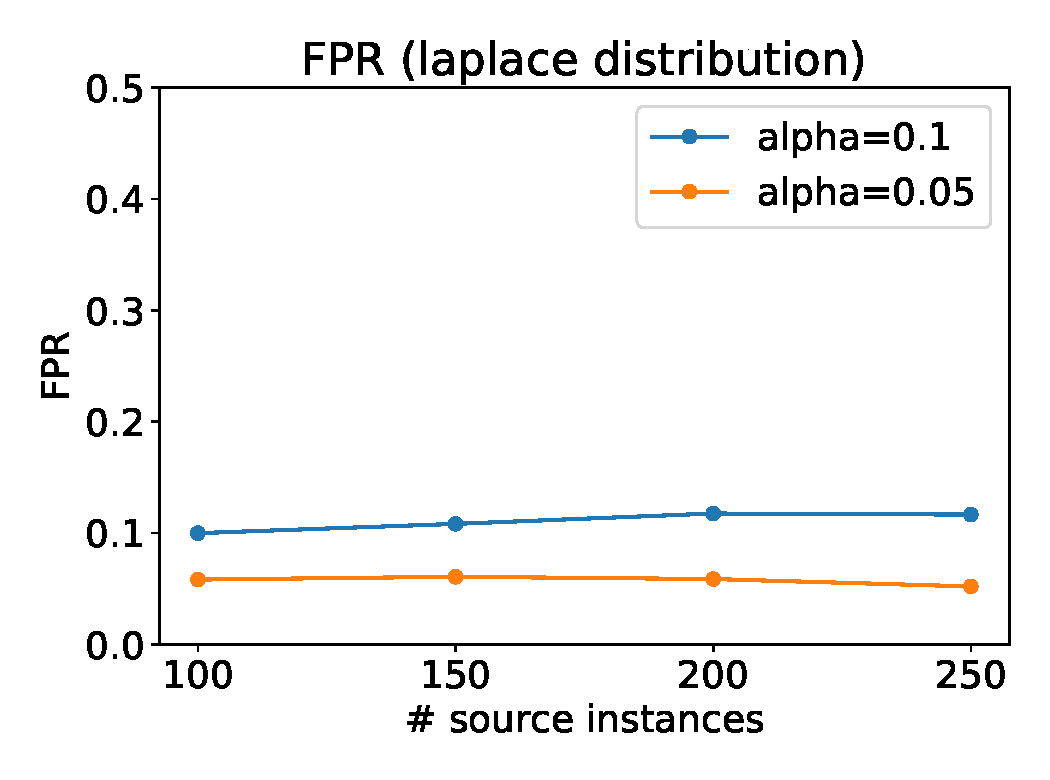
\includegraphics[width=\linewidth]{robust_laplace}
\caption{Laplace distribution}
\label{fig:app_laplace}
\end{subfigure}
%
\begin{subfigure}{0.3\linewidth}
\centering
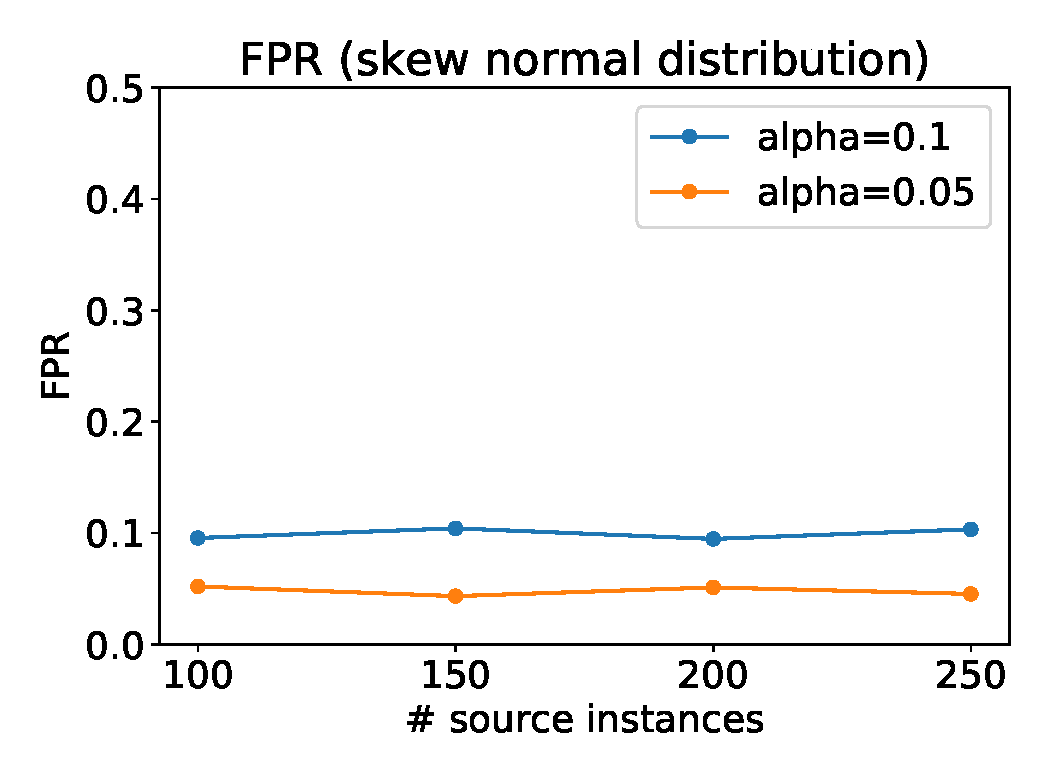
\includegraphics[width=\linewidth]{robust_skew}
\caption{Skew normal distribution}
\label{fig:app_skew_normal}
\end{subfigure}

\begin{subfigure}{0.3\linewidth}
\centering
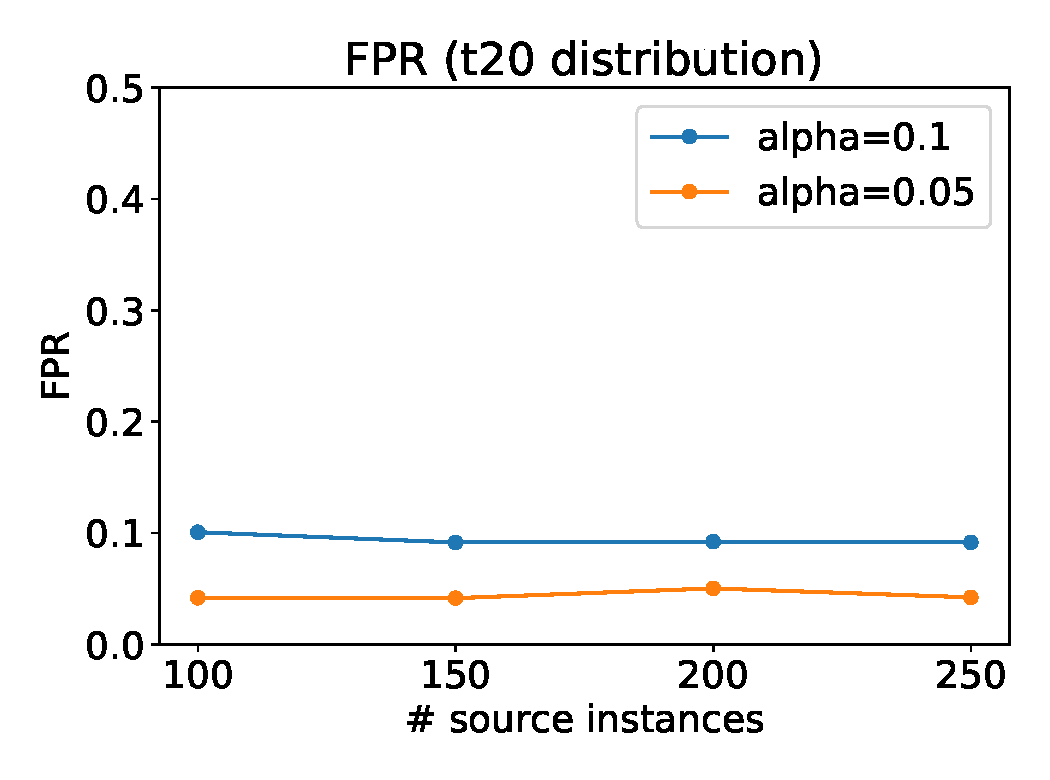
\includegraphics[width=\linewidth]{robust_t20}
\caption{$t_{20}$ distribution}
\label{fig:app_t_20}
\end{subfigure}
%
\begin{subfigure}{0.3\linewidth}
\centering
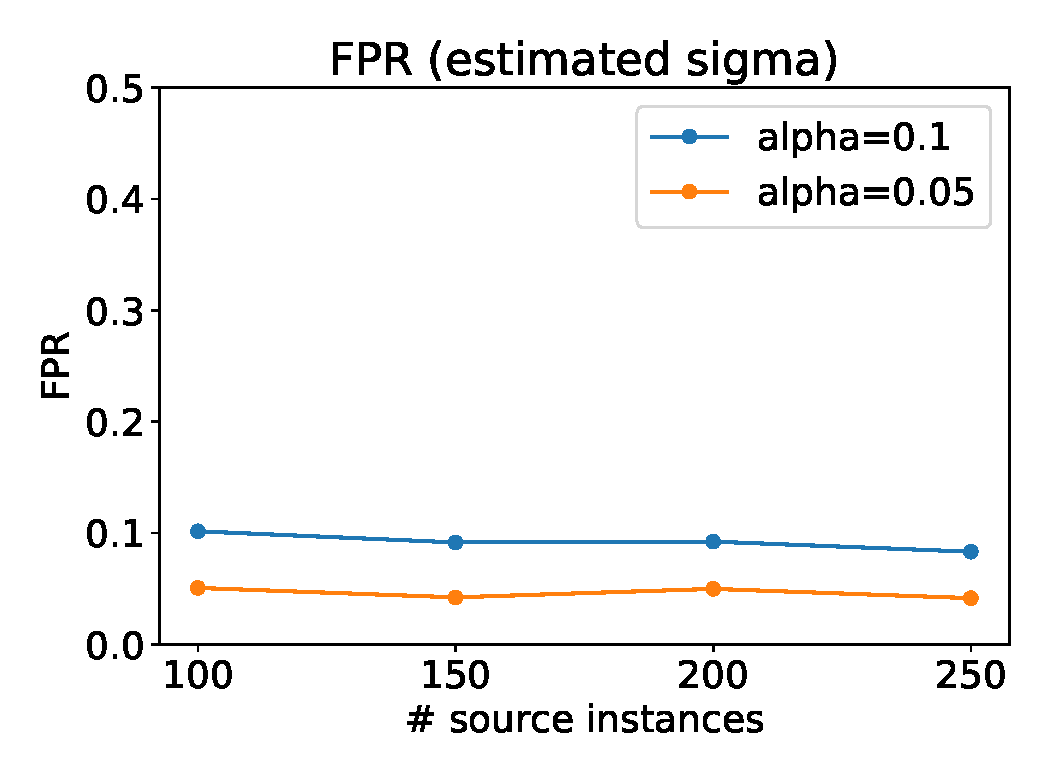
\includegraphics[width=\linewidth]{robust_estimated_sigma}
\caption{Estimated variance}
\label{fig:app_unknown_sigma}
\end{subfigure}
\caption{False positive rate of the proposed {\tt CAD-DA} method when data is non-normal or variance is unknown.}
\label{fig:violate_assumption}
\end{figure}







